\documentclass[
  bibliography=totoc,     % Literatur im Inhaltsverzeichnis
  captions=tableheading,  % Tabellenüberschriften
  titlepage=firstiscover, % Titelseite ist Deckblatt
  DIV=16
]{scrartcl}

% Paket float verbessern
\usepackage{scrhack}

% Seitenränder etc.
%\usepackage[a4paper]{geometry}

% Warnung, falls nochmal kompiliert werden muss
\usepackage[aux]{rerunfilecheck}

% deutsche Spracheinstellungen
\usepackage{polyglossia}
\setmainlanguage{german}

\usepackage{sourceserifpro}
\usepackage{sourcesanspro}
%\usepackage{charter}

% unverzichtbare Mathe-Befehle
\usepackage{amsmath}
% viele Mathe-Symbole
\usepackage{amssymb}
% Erweiterungen für amsmath
\usepackage{mathtools}


% Fonteinstellungen
\usepackage{fontspec}
% Latin Modern Fonts werden automatisch geladen

\usepackage[
  math-style=ISO,    % ┐
  bold-style=ISO,    % │
  sans-style=italic, % │ ISO-Standard folgen
  nabla=upright,     % │
  partial=upright,   % ┘
  warnings-off={           % ┐
    mathtools-colon,       % │ unnötige Warnungen ausschalten
    mathtools-overbracket, % │
  },                       % ┘
]{unicode-math}


% traditionelle Fonts für Mathematik
%\setmainfont{SourceSerifPro}
%\setmathfont{Latin Modern Math}
%\setmathfont{XITS Math}[range={scr, bfscr}]
%\setmathfont{XITS Math}[range={cal, bfcal}, StylisticSet=1]

% Zahlen und Einheiten
\usepackage[
  locale=DE,                 % deutsche Einstellungen
  separate-uncertainty=true, % immer Fehler mit \pm
  per-mode=reciprocal,       % ^-1 für inverse Einheiten
%  output-decimal-marker=.,   % . statt , für Dezimalzahlen
]{siunitx}

% chemische Formeln
\usepackage[
  version=4,
  math-greek=default, % ┐ mit unicode-math zusammenarbeiten
  text-greek=default, % ┘
]{mhchem}

% richtige Anführungszeichen
\usepackage[autostyle]{csquotes}

% schöne Brüche im Text
\usepackage{xfrac}

% Standardplatzierung für Floats einstellen
\usepackage{float}
\floatplacement{figure}{htbp}
\floatplacement{table}{htbp}

% Floats innerhalb einer Section halten
\usepackage[
  section, % Floats innerhalb der Section halten
  below,   % unterhalb der Section aber auf der selben Seite ist ok
]{placeins}

% Captions schöner machen.
\usepackage[
  labelfont=bf,        % Tabelle x: Abbildung y: ist jetzt fett
  font=small,          % Schrift etwas kleiner als Dokument
  width=0.9\textwidth, % maximale Breite einer Caption schmaler
]{caption}
% subfigure, subtable, subref
\usepackage{subcaption}

% Grafiken können eingebunden werden
\usepackage{graphicx}
% größere Variation von Dateinamen möglich
\usepackage{grffile}

% schöne Tabellen
\usepackage{booktabs}

% Verbesserungen am Schriftbild
\usepackage{microtype}

% Literaturverzeichnis
%\usepackage[
%  backend=biber,
%  sorting=none
%]{biblatex}

% Hyperlinks im Dokument
\usepackage[
  unicode,        % Unicode in PDF-Attributen erlauben
  pdfusetitle,    % Titel, Autoren und Datum als PDF-Attribute
  pdfcreator={},  % ┐ PDF-Attribute säubern
  pdfproducer={}, % ┘
]{hyperref}
% erweiterte Bookmarks im PDF
\usepackage{bookmark}

% Trennung von Wörtern mit Strichen
\usepackage[shortcuts]{extdash}

\usepackage[shortlabels]{enumitem}

\usepackage{braket}

\DeclareMathOperator{\Tr}{Tr}
\usepackage[makeroom]{cancel}

%Eigene Befehle
\ExplSyntaxOn
\NewDocumentCommand \fig {mmmO{}}
{
  \begin{figure}
    \centering
    \includegraphics[#4]{#1}
    \caption{#2}
    \label{fig:#3}
  \end{figure}
}
\ExplSyntaxOff


\author{Jasper Karl Lammering\\Henning Ptaszyk\\Timo Gräßer}
\subtitle{Computational Physics}


\usepackage{listings}
\usepackage[dvipsnames]{xcolor}

\title{Blatt 8}
\date{
  Abgabe: \today
}

\begin{document}
\maketitle
Wir stimmen für die mündliche Prüfung.

Alle Dateien ausführbar mit der Makefile. %Der Output wird dann in die Datei\texttt{blatt2\_ausgabe.txt} geschrieben.
\section*{Aufgabe 1}
\subsection*{a) , b)}
\begin{figure}
  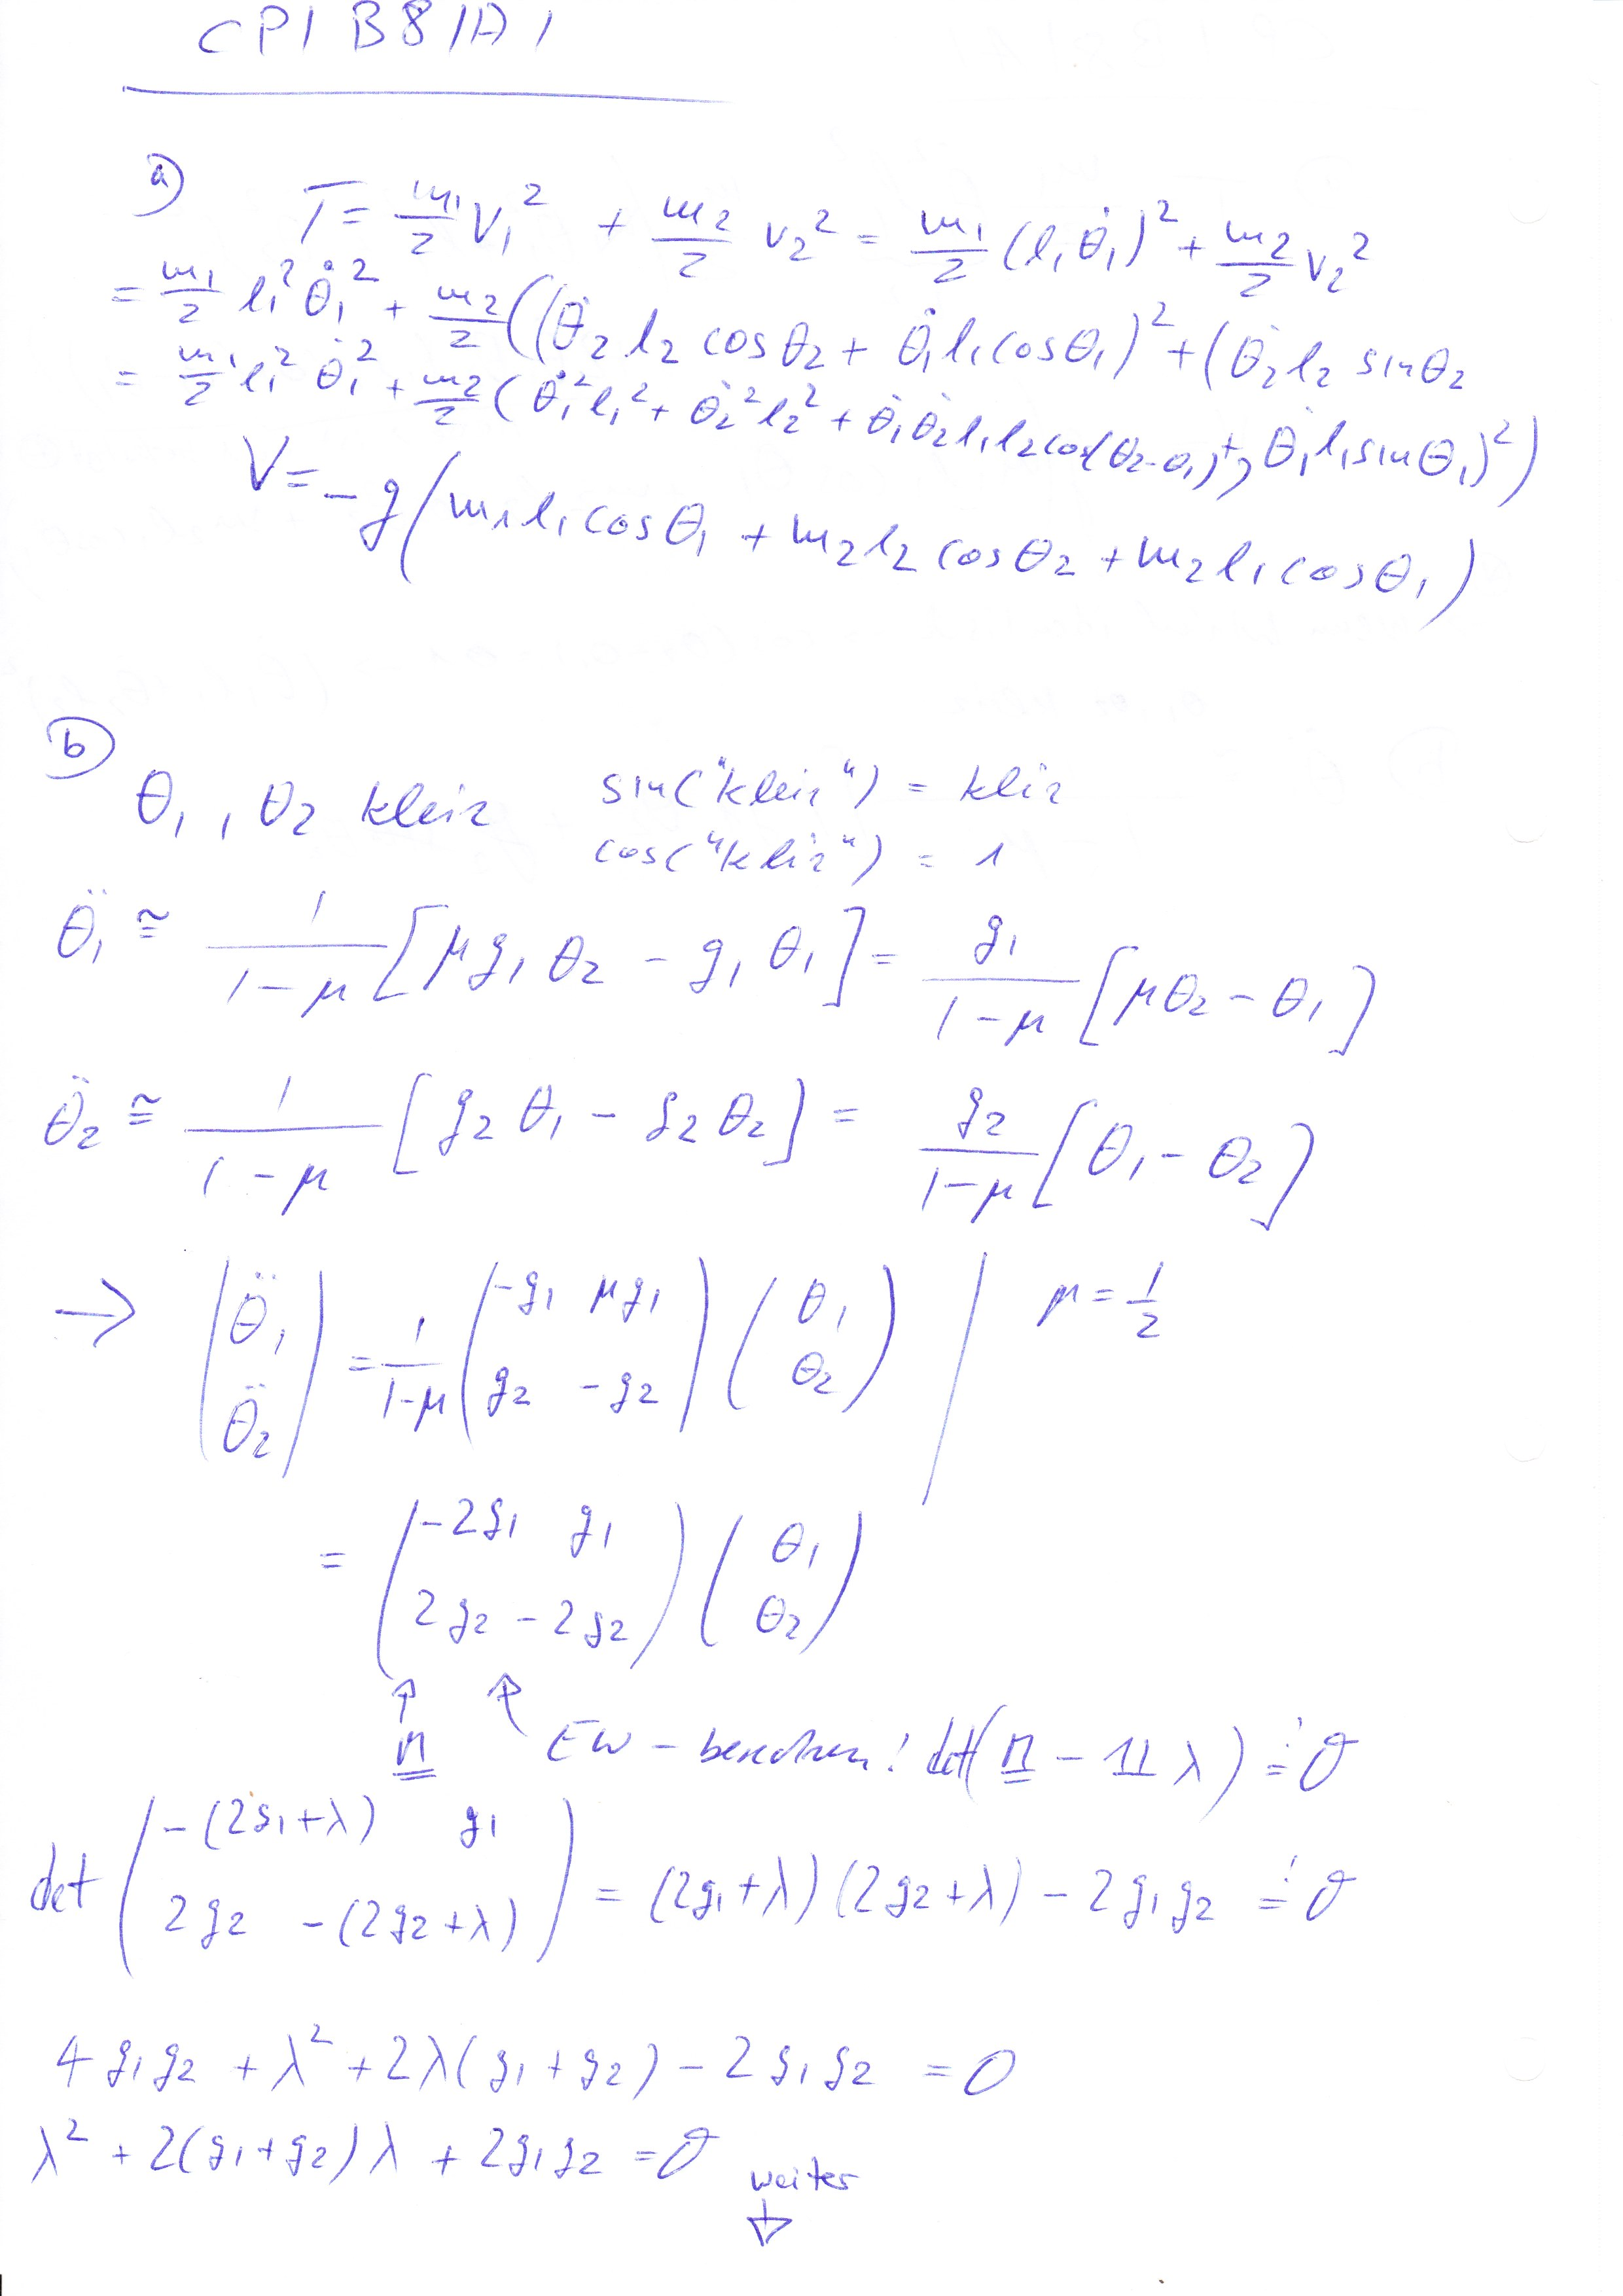
\includegraphics[width=\textwidth]{cp_8_11.jpg}
  \caption{Aufgabe 1 a) und b) (1/2).}
  \label{fig:bild1}
\end{figure}


\begin{figure}
  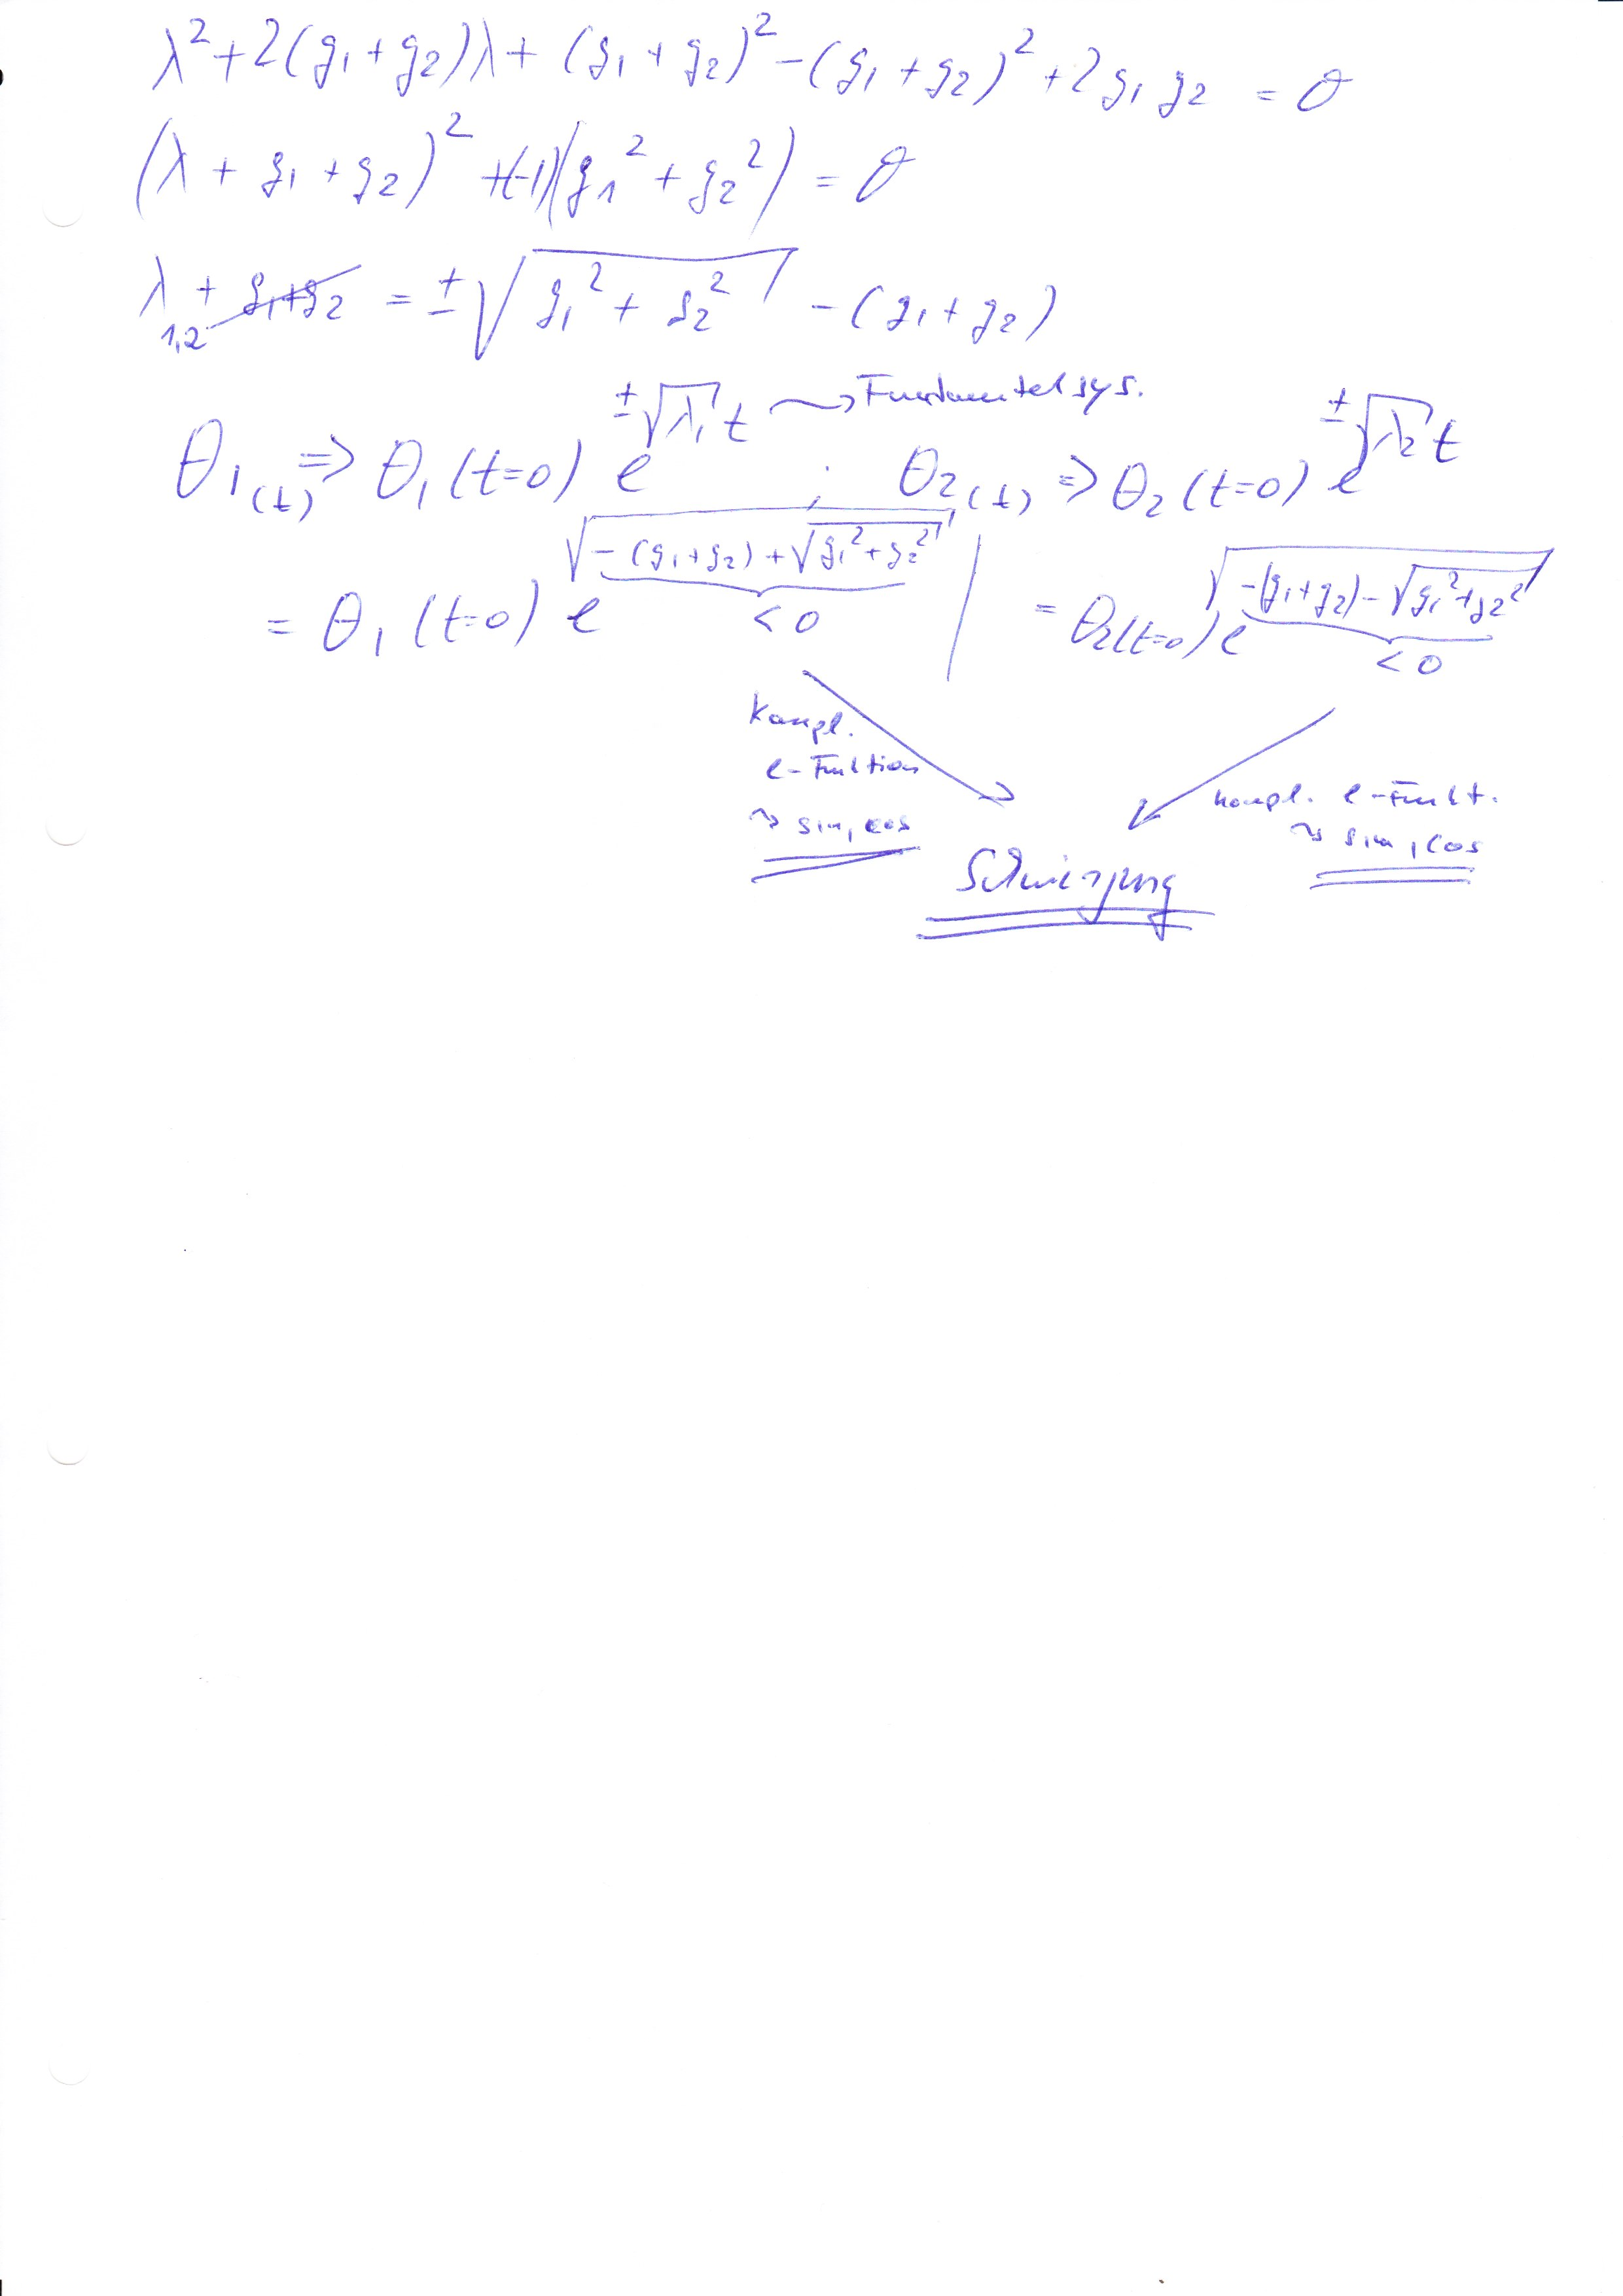
\includegraphics[width=\textwidth]{cp_8_12.jpg}
  \caption{Aufgabe 1 a) und b) (2/2).}
  \label{fig:bild2}
\end{figure}

\FloatBarrier
\subsection*{c)}

Energieerhaltung nicht so ganz gegeben.
(Haben den (Tipp-)Fehler leider nicht gefunden.)

\begin{figure}
  \includegraphics[width=\textwidth]{build/energie.pdf}
  \caption{Aufgabe 1 c) 1. startbedingung.}
  \label{fig:bild3}
\end{figure}

\begin{figure}
  \includegraphics[width=\textwidth]{build/energie.pdf}
  \caption{Aufgabe 1 c) 2. startbedingung.}
  \label{fig:bild4}
\end{figure}


\begin{figure}
  \includegraphics[width=\textwidth]{build/1.pdf}
  \caption{Aufgabe 1 c) 1. startbedingung.}
  \label{fig:bild5}
\end{figure}

\begin{figure}
  \includegraphics[width=\textwidth]{build/2.pdf}
  \caption{Aufgabe 1 c) 2. startbedingung.}
  \label{fig:bild5}
\end{figure}


Animationen(.mp4) werden mit \textit{make} erstellt.



\end{document}
